%-----------------------------------------------%
% Plano de Aula 01
%-----------------------------------------------%
\begin{anexosenv}     
    % \chapter{Acompanhamento de Aulas}
    % \begin{landscape}    
    % \end{landscape}
    % \chapter{Cronograma de aulas}
    % 	\includepdf[pages=-]{03-pos-textual/cronograma.pdf}
    \chapter{Materiais da Turma}
    \label{anx:materiaisAnexo}
    
    \section{Unidade: Dilatação Térmica}
    \label{sec:materialAnexoDilatacaoTermica}
    Material de apoio desenvolvido pelo professor supervisor, para suporte às aulas de Dilatação Térmica. Este material encontra-se disponível para a turma no ambiente de ensino virtual \emph{Google Classroom} destacado pelo retângulo em vermelho na \autoref{fig:gClassroom}
    \vspace{1cm}
    \begin{figure}[!h]
        \centering
        \footnotesize
        \caption{Print Screen do Google Classroom da Turma 2(7)}
        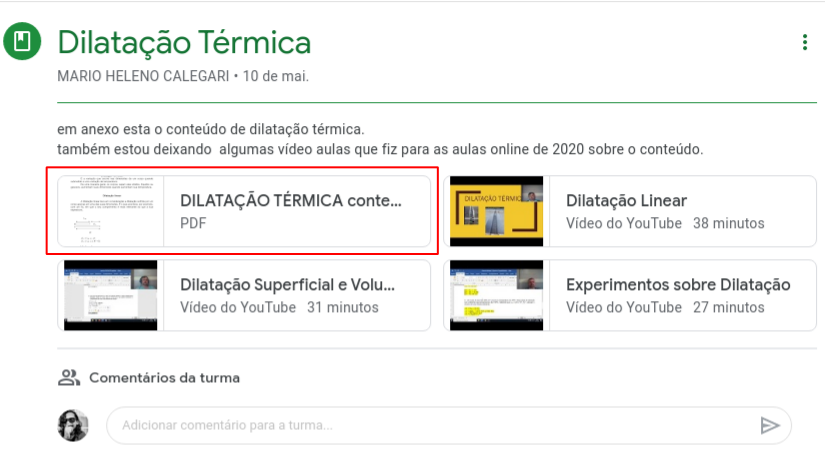
\includegraphics[width=\textwidth]{03-elementos/03.2_textual/03.2.1_fig/google-class01.png}
        \label{fig:gClassroom}
    \end{figure}

    Segue na integra:
    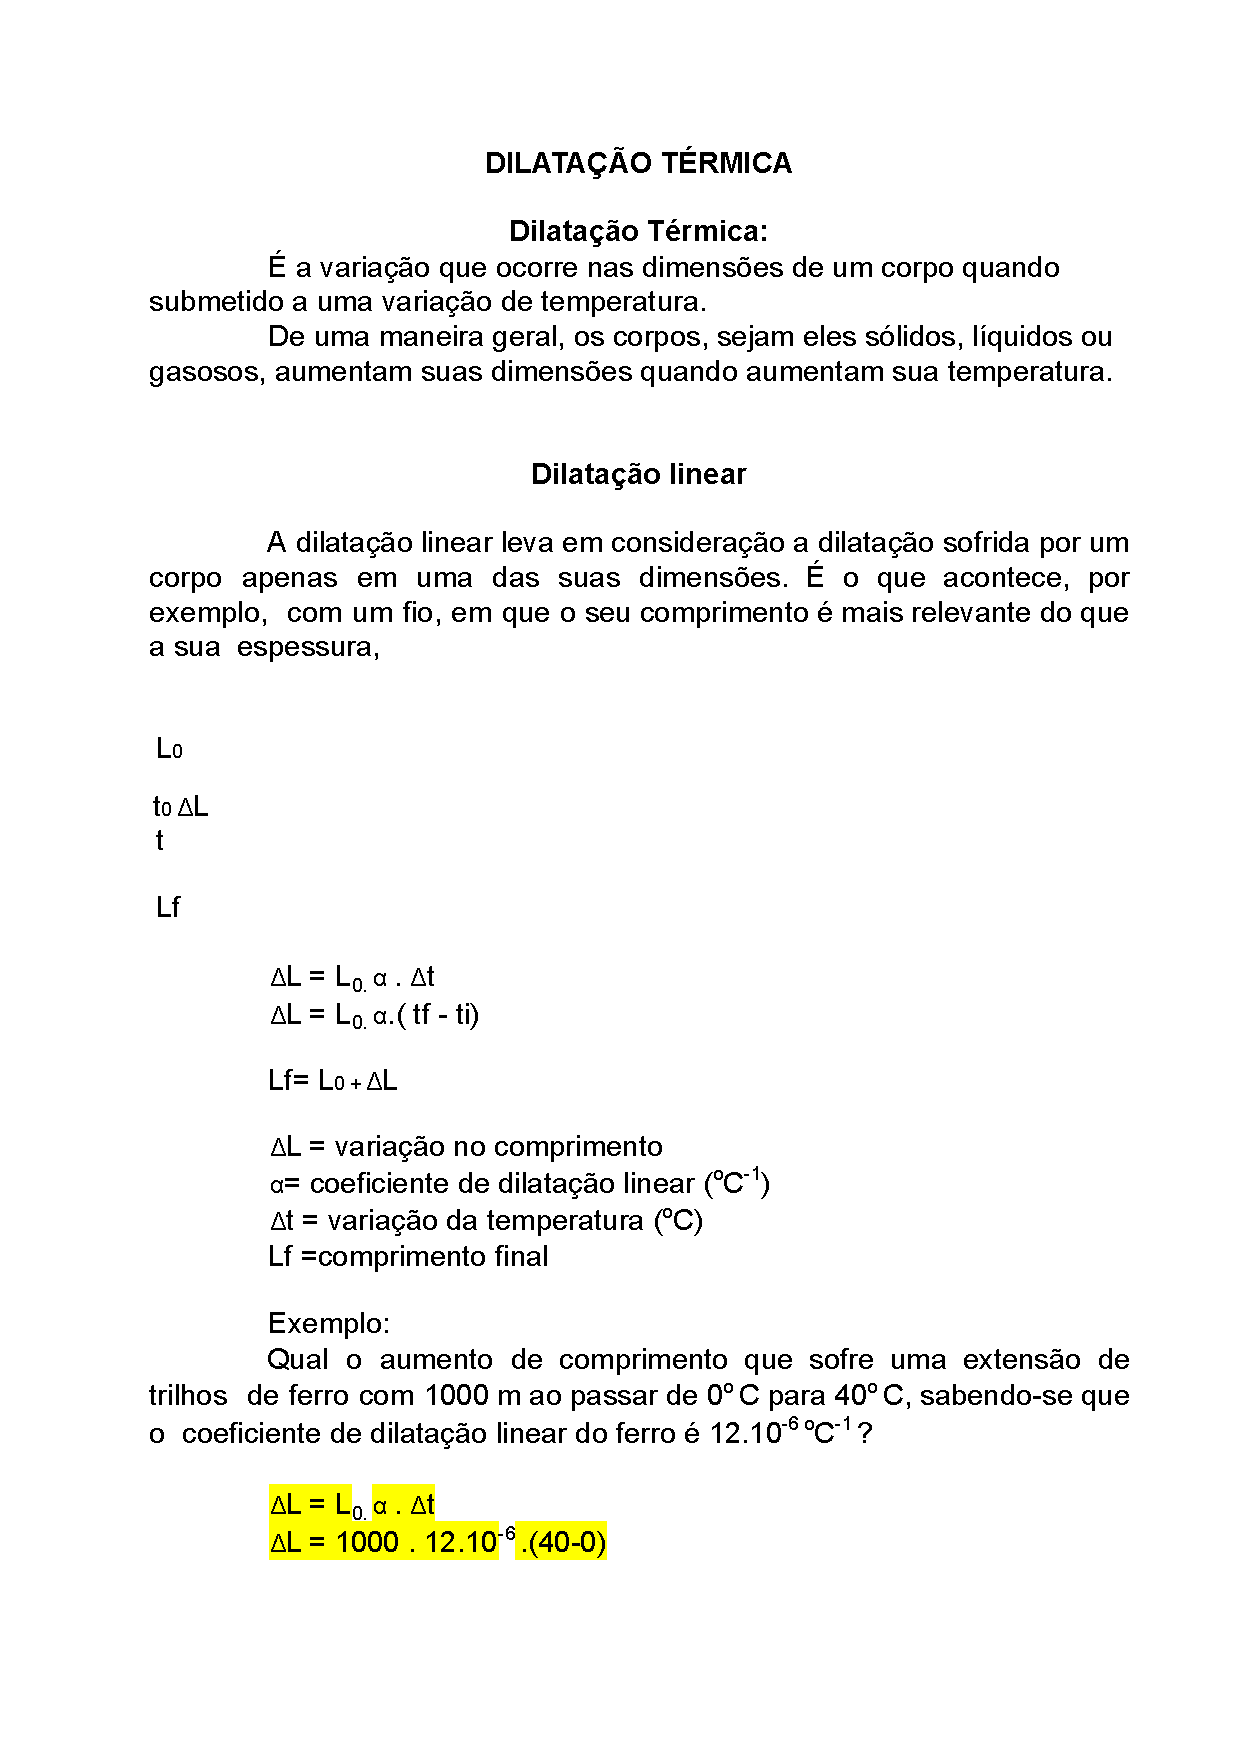
\includepdf[pages=-,scale=1]{03-elementos/03.2_textual/03.2.1_fig/apendice-I}
    \includecode[shell]{l_olamundo}{Olá mundo em shell script}{03-elementos/03.2_textual/03.2.0_codes/ola.sh}   
\end{anexosenv}
